%%%%%%%%%%%%%%%%%%%%%%%%%%%%%%%%%%%%%%%%%%%%%%%%%%%%%%
% This is beamer setup. Not required for extraction. I personnaly like the default barebones style.
\documentclass{beamer}
\usepackage[utf8]{inputenc}
\usetheme{default}

%%%%%%%%%%%%%%%%%%%%%%%%%%%%%%%%%%%%%%%%%%%%%%%%%%%%%%
\usepackage{tikz}\usetikzlibrary{calc}
\usepackage{bbm}
\usepackage{amsmath}
\usepackage{hyperref}
\usepackage{bm} % bold math mode

\usepackage{minted}
\setminted{fontsize=\footnotesize}

\usepackage{pdfpages} % import slides from Patricia

\newcommand\D{\mathrm{d}}
\newcommand\R{\mathbbm{R}}

\newcommand\Convolution{\ast}
\newcommand\Correlation{\star}

\newcommand\Reversed[1]{\overline{#1}}
\newcommand\Indicator[1]{\mathbbm{1}_{#1}}

\DeclareMathOperator{\nzd}{nzd}
\DeclareMathOperator{\IntervalLeft}{left}
\DeclareMathOperator{\IntervalRight}{right}
\DeclareMathOperator{\IntervalCenter}{center}
\DeclareMathOperator*{\argmin}{arg\,min}

%%%%%%%%%%%%%%%%%%%%%%%%%%%%%%%%%%%%%%%%%%%%%%%%%%%%%%

\title{Calcul d'intégrales pour processus de Hawkes}
\author{François Gindraud \\ avec Anna Bonnet et Franck Picard}
\date{14 juin 2022}

\begin{document}

\maketitle

% Hawkes process, from slides of Patricia
{
    \setbeamercolor{background canvas}{bg=}
    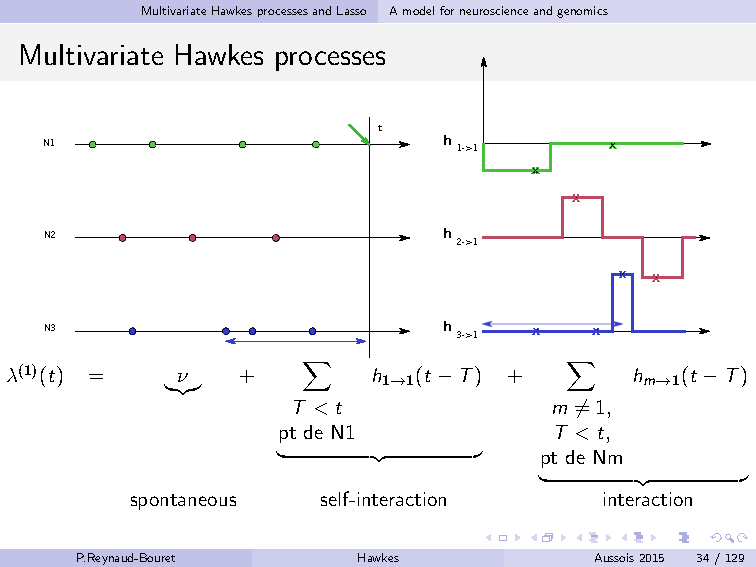
\includepdf{pg_0113.pdf}
}

\begin{frame}\frametitle{Function basis decomposition}
\[ h_{l \rightarrow m}(t - T) = \sum_{0 \le k < K} a_{k,l \rightarrow m} \varphi_k(t - T) \]

\begin{columns}
    \begin{column}{0.4\textwidth}
        \textbf{Histograms}
        \small\[ \varphi_k = \frac{1}{\sqrt{\delta}} \mathbbm{1}_{]k\delta, (k+1)\delta]} \]
        \begin{center}\begin{tikzpicture}
            \draw[->] (0,-0.5) -- (0, 3);
            \node[below right] at (0, 0) {$0$};
            \draw[dashed] (0,0) -- (1,0) node[below] {$\delta$};
            \draw[color=blue] (-0.3,0) node[left]{$\varphi_0$} -| (0,0.7) -| (1,0) -- (3.5,0);
            \draw[dashed] (1,1) -- (2,1);
            \draw[color=green] (-0.3,1) node[left]{$\varphi_1$} -| (1,1.7) -| (2,1) -- (3.5,1);
            \draw[dashed] (2,2) -- (3,2);
            \draw[color=red] (-0.3,2) node[left]{$\varphi_2$} -| (2,2.7) -| (3,2) -- (3.5,2);
        \end{tikzpicture}\end{center}
    \end{column}
    \begin{column}{0.6\textwidth}
        \textbf{Haar Wavelets}
        \small\[
            \varphi_{s,p} = \frac{\sqrt{2}^s}{\sqrt{\delta}} \left(
            \Indicator{ \left] \frac{2p \delta}{2^{s+1}}, \frac{(2p+1) \delta}{2^{s+1}} \right] } -
            \Indicator{ \left] \frac{(2p +1) \delta}{2^{s+1}}, \frac{(2p + 2) \delta}{2^{s+1}} \right] }
            \right)
        \]
        \small \[ 0 \le s < \text{Nscale} \qquad 0 \le p < 2^s \]
        \begin{center}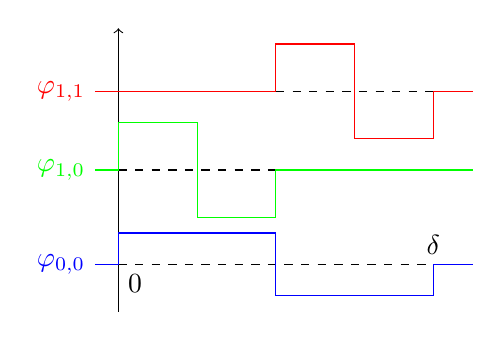
\begin{tikzpicture}
            \draw[->] (0,-0.6) -- (0, 3);
            \node[below right] at (0, 0) {$0$};
            \draw[dashed] (0,0) -- (4,0) node[above] {$\delta$};
            \draw[color=blue] (-0.3,0) node[left]{$\varphi_{0,0}$} -| (0,0.4) -| (2,-0.4) -| (4,0) -- (4.5,0);
            \draw[dashed] (0,1.2) -- (2,1.2);
            \draw[color=green] (-0.3,1.2) node[left]{$\varphi_{1,0}$} -| (0,1.8) -| (1,0.6) -| (2,1.2) -- (4.5,1.2);
            \draw[dashed] (2,2.2) -- (4,2.2);
            \draw[color=red] (-0.3,2.2) node[left]{$\varphi_{1,1}$} -| (2,2.8) -| (3,1.6) -| (4,2.2) -- (4.5,2.2);
        \end{tikzpicture}\end{center}
    \end{column}
\end{columns}
\end{frame}

\begin{frame}\frametitle{Inferrence optimization problem (Lasso)}
\begin{tikzpicture}
    \node (lasso) at (0,0) {$\displaystyle \widehat{\bm{a}} = \argmin_{\bm{a}} \bm{a}^\intercal \bm{G} \bm{a} - 2 \bm{a}^\intercal \bm{B} + \lambda \bm{d}^\intercal |\bm{a}|$};
    \draw[->] ($(lasso)+(2.7,0.3)$) |- ++(1,0.2) node[right] {$\left[ a_{k,l \rightarrow m} \right] : float[k \times l \times m]$};
    \draw[->] ($(lasso)+(1.2,-0.1)$) |- ++(-4,-0.6) |- ++(0.3,-0.9) node[right] {$\displaystyle
        b_{k,l \rightarrow m} = \sum_{X_l \in N_l, X_m \in N_m} \varphi_k (X_m - X_l)
    $};
    \draw[->] ($(lasso)+(-0.35,-0.1)$) |- ++(-2.7,-0.4) |- ++(0.5,-2.5) node[right] {$\displaystyle
        G_{l,l',k,k'} = \int_\R \left( \sum_{X_l \in N_l} \varphi_k(x-X_l) \right) \left( \sum_{X_{l'} \in N_{l'}} \varphi_{k'}(x-X_{l'}) \right) \D x
    $};
    \draw[->] ($(lasso)+(2.2,-0.1)$) |- ++(6,-0.4) |- ++(-3.5,-5) node[left] (D) {$\displaystyle
        \left. \begin{aligned}
            \widehat{v}_{k,l \rightarrow m} & = \sum_{X_m \in N_m} \left( \sum_{X_l \in N_l} \varphi_k(X_m-X_l) \right)^2 \\
            \widehat{b}_{k,l \rightarrow m} & = \sup_x \left|\sum_{X_l \in N_l} \varphi_k(x - X_l) \right| \\
        \end{aligned} \right\}
    $};
\end{tikzpicture}
\end{frame}

\begin{frame}[fragile]\frametitle{General optimizations}
    Symmetries
    \[ G_{l,l',k,k'} = G_{l',l,k',k} \]
    
    Factoring scaling out : dealing with $\Indicator{[a,b]}$ is easier
    \begin{minted}[]{C++}
template<typename Inner> double compute(const Scaled<Inner> & shape) {
    return shape.scale * compute(shape.inner);
}
double compute(const Indicator & ind) { ... }
using Histogram = Scaled<Indicator>;
    \end{minted}
    
    Shifting invariance with histograms
    \begin{itemize}
        \item $G_{l,l',k,k'} = G_{l,l',k+c,k+'c}$ (using $x \rightarrow x + \delta c$)
        \item $\widehat{b}_{k,l \rightarrow m} = \sup_x \left|\sum_{X_l \in N_l} \varphi_k(x - X_l) \right|$ independent of $m$ or $k$
    \end{itemize}
\end{frame}

\begin{frame}\frametitle{$\bm{B}$ and $\widehat{\bm{V}}$ using sliding windows}
    \[ \Indicator{x} \]
    Sliding window over points to go from quadratic to approximately linear.

    TODO
\end{frame}

\begin{frame}\frametitle{$\widehat{\bm{B}}$ sup by enumerating function values}
    $\sup_x \left|\sum_{X_l \in N_l} \Indicator{I}(x - X_l) \right| $ can be evaluated exactly.

    Enumerate point of change.

    TODO
\end{frame}

\begin{frame}\frametitle{$G_{l,l',k,k'}$ expressed using function correlation}
    \[ \begin{split}
        \mathsf{G}_{l,l',k,k'}
        & = \int \left( \sum_{X_l \in N_l} \varphi_k(x-X_l) \right) \left( \sum_{X_{l'} \in N_{l'}} \varphi_{k'}(x-X_{l'}) \right) \D x \\
        & = \sum_{X_l \in N_l, X_{l'} \in N_{l'}} \int \varphi_k(x-X_l) \varphi_{k'}(x-X_{l'}) \D x \\
        & = \sum_{X_l \in N_l, X_{l'} \in N_{l'}} \int \varphi_k(x-(X_l-X_l')) \varphi_{k'}(x) \D x \\
        & = \sum_{X_l \in N_l, X_{l'} \in N_{l'}} [\varphi_k \Correlation \varphi_{k'}] (X_l-X_l')
    \end{split} \]
    In the form $\sum_{X_m \in N_m, X_l \in N_l} F(X_l - X_m)$ so we can reuse the strategy used for $\bm{B}$.
\end{frame}

\begin{frame}\frametitle{Convolution, correlation}
    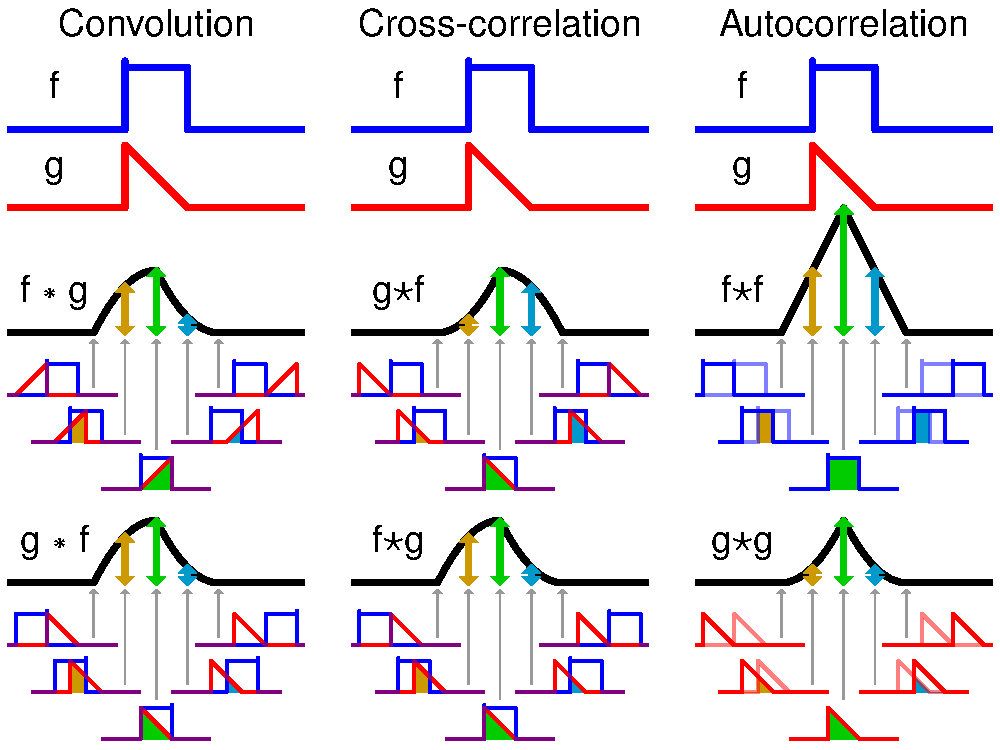
\includegraphics[width=\textwidth]{wikipedia_convolution_correlation}
\end{frame}

\begin{frame}\frametitle{Properties}
    Shift, reversal, etc.
\end{frame}

\begin{frame}\frametitle{Trapezoid}
    Derive computation for Indicator self correlated
\end{frame}

\begin{frame}\frametitle{Computation strategy summary}

    B, G, V hat use sum of point differences.
    B hat use exact sup.

    Use symmetries and simplifications.
    
    Complexities, basic benchmark.

\end{frame}

%%%% Kernel starts !

\begin{frame}\frametitle{Kernel version}
    Replace $\varphi_k$ by $\varphi_k \Convolution \eta_l$.
    
    New values of B,G,B hat, V hat.
\end{frame}

\begin{frame}\frametitle{Shape strategy}
    Introduce trapezoid decomposition.

    Need to introduce more shapes with higher order polynomials, works but tedious to do computations.
    Rigid for future use (new kernels like $x^2$ approx of gaussian, etc).
\end{frame}

\begin{frame}\frametitle{Generalization}
    Introduce polynom on interval.

    Basic props with respect to shifting and reversing.
\end{frame}

\begin{frame}\frametitle{Convolution of polynomial}
    Convolution : 3 pieces of polynomials with specific degrees.

    Add one formula for the fun.

    Distributes when convolution of sum of polynomials.
\end{frame}

\begin{frame}\frametitle{Properties / implementation}
    Automatic convolution computation.

    Demo of dump shapes.

    Debug capabilities : must be continuous.

    Choice of evaluation from center to reduce numerical error.

    Still costly due to quick explosion of degree.

    Other operators : cut to positive support (recenter polynoms and recompute coefficients).
\end{frame}

\begin{frame}\frametitle{And the sup ?}
    Must approximate.

    In case of histograms, using an approximation with indicator scaled to average polynom value.
    Average computed automatically using integral.

    In practice the sup was supposed to become negligible, not always though.
    Better strategies could be devised.
\end{frame}

\begin{frame}\frametitle{Final strategy}

    B, G, V hat using shapes and symmetries.

    B hat approx sup.

\end{frame}

\end{document}